\newcommand*{\includesDirectory}{includes}
\newcommand*{\settingsDirectory}{\includesDirectory/settings}
\newcommand*{\plotsDirectory}{\includesDirectory/plots}

\documentclass[a4paper,12pt,oneside]{book}
\usepackage{geometry}

\usepackage{setspace}
\usepackage{listings}
\usepackage{graphicx}

\usepackage{xcolor}

\definecolor{codegreen}{rgb}{0,0.6,0}
\definecolor{codegray}{rgb}{0.5,0.5,0.5}
\definecolor{codepurple}{rgb}{0.58,0,0.82}
\definecolor{backcolour}{rgb}{0.95,0.95,0.92}

\lstdefinestyle{mystyle}{
    backgroundcolor=\color{backcolour},   
    commentstyle=\color{codegreen},
    keywordstyle=\color{magenta},
    numberstyle=\tiny\color{codegray},
    stringstyle=\color{codepurple},
    basicstyle=\ttfamily\footnotesize,
    breakatwhitespace=false,         
    breaklines=true,                 
    captionpos=b,                    
    keepspaces=true,                 
    numbers=left,                    
    numbersep=5pt,                  
    showspaces=false,                
    showstringspaces=false,
    showtabs=false,                  
    tabsize=2
}
\usepackage{float}
\lstset{style=mystyle}


\geometry{
    left=  20mm,
    right= 20mm,
    top=   20mm,
    bottom=20mm
}

\setlength{\parindent}{0mm}

\usepackage{array}

\usepackage[T1]{fontenc}
\usepackage[polish]{babel}
\usepackage{lmodern}
\usepackage{titletoc}
\usepackage{hyperref}
\usepackage[all]{hypcap}
\setcounter{tocdepth}{1}

\renewcommand\thechapter{Rozdział \Roman{chapter}}
\renewcommand\thesection{\arabic{section}.}
\renewcommand\thesubsection{\arabic{section}.\arabic{subsection}}
\contentsmargin{0.5cm}
\newlength\chapterlength
\settowidth\chapterlength{\hspace{2.5cm}}

\titlecontents{chapter}
    [\chapterlength] %5.3
    {\vspace{0.2cm}}
    {\contentslabel[\thecontentslabel]{\chapterlength}}%\thecontentslabel
    {\hspace*{-\chapterlength}}% unnumbered chapters
    {\titlerule*[1cm]{.}\contentspage}[\vspace{0.2cm}]%

\titlecontents{section}
    [\chapterlength] %5.3
    {\small}
    {\contentslabel[\thecontentslabel]{0.5cm}}
    {}
    {\titlerule*[0.5cm]{.}\contentspage}[]




\usepackage{titlesec}


\titleformat{\chapter}[block]
  {\normalfont}
  {\Huge{\thechapter\vspace{-13pt}\\}}
  {0pt}
  {\Large}
\titlespacing*{\chapter}{0pt}{0pt}{10pt}

\newcommand{\chapterwithout}[1]{\chapter*{#1} 
\addcontentsline{toc}{chapter}{#1}  
}

\titleformat{\section}
  {\normalfont}
  {\makebox[0.5cm][l]{\thesection}}
  {10pt}
  {}
\titlespacing*{\section}{0pt}{10pt}{10pt}

\titleformat{\subsection}[block]
  {\normalfont}
  {\hspace{1cm}\makebox[0.5cm][l]{\thesubsection}}{10pt}{}
\titlespacing*{\subsection}{0pt}{5pt}{5pt}

\renewcommand{\labelenumi}{$\arabic{enumi}^\circ$}


\begin{document}
	\thispagestyle{empty}
	\vspace*{\fill}
			\begin{center}
				\Huge{
					\textit{\texttt{PROJEKT JĘZYK R}}
				}
			\end{center}
	\vspace*{\fill}
			\begin{tabular}{ll}
				\texttt{zbiór danych:}  & \texttt{Video Game Sales \cite{source}}\\
				\texttt{autor:}         & \texttt{Marcin Belicki}\\
				\texttt{numer indeksu:} & \texttt{273417}
			\end{tabular}
	\newpage
	\setlength{\parindent}{9mm}
	
	\section{Opis zbioru danych}
		Zbiór danych zawiera listę gier ze sprzedażą przekraczającą 100 000 kopii. Dane zostały pozyskane ze strony \href{https://www.vgchartz.com/}{vgchartz.com}.\\
		Opisy poszczególnych pól:\vspace{0.2cm}\\
	\begin{tabular}{> {\ttfamily}l l}
		Rank          & ranga gry pod względem sprzedaży ogółem\\
		Name          & nazwa gry\\
		Platform      & platforma, na którą gra została wydana (np. PC, PS4 itp.)\\
		Year          & rok wydania gry\\
		Genre         & gatunek gry\\
		Publisher     & wydawca gry\\
		NA\_Sales     & liczba sprzedanych kopii w Ameryce Północnej (w milionach)\\
		EU\_Sales     & liczba sprzedanych kopii w Europie (w milionach)\\
		JP\_Sales     & liczba sprzedanych kopii w Japonii (w milionach)\\
		Other\_Sales  & liczba sprzedanych kopii w reszcie świata (w milionach)\\
		Global\_Sales & liczba sprzedanych kopii na całym świecie (w milionach) - zmienna główna
	\end{tabular}\\
	Import danych został do środowiska R zostł wykonany za pomocą kodu:
	\begin{lstlisting}[language=R]
	data = read.csv("vgsales.csv", sep = ",")
	
	list2env(data ,.GlobalEnv)
\end{lstlisting}
	
	\section{Ilustracja graficzna zmiennej głównej}
	
	\begin{center}
	\begin{figure}[h!]
  	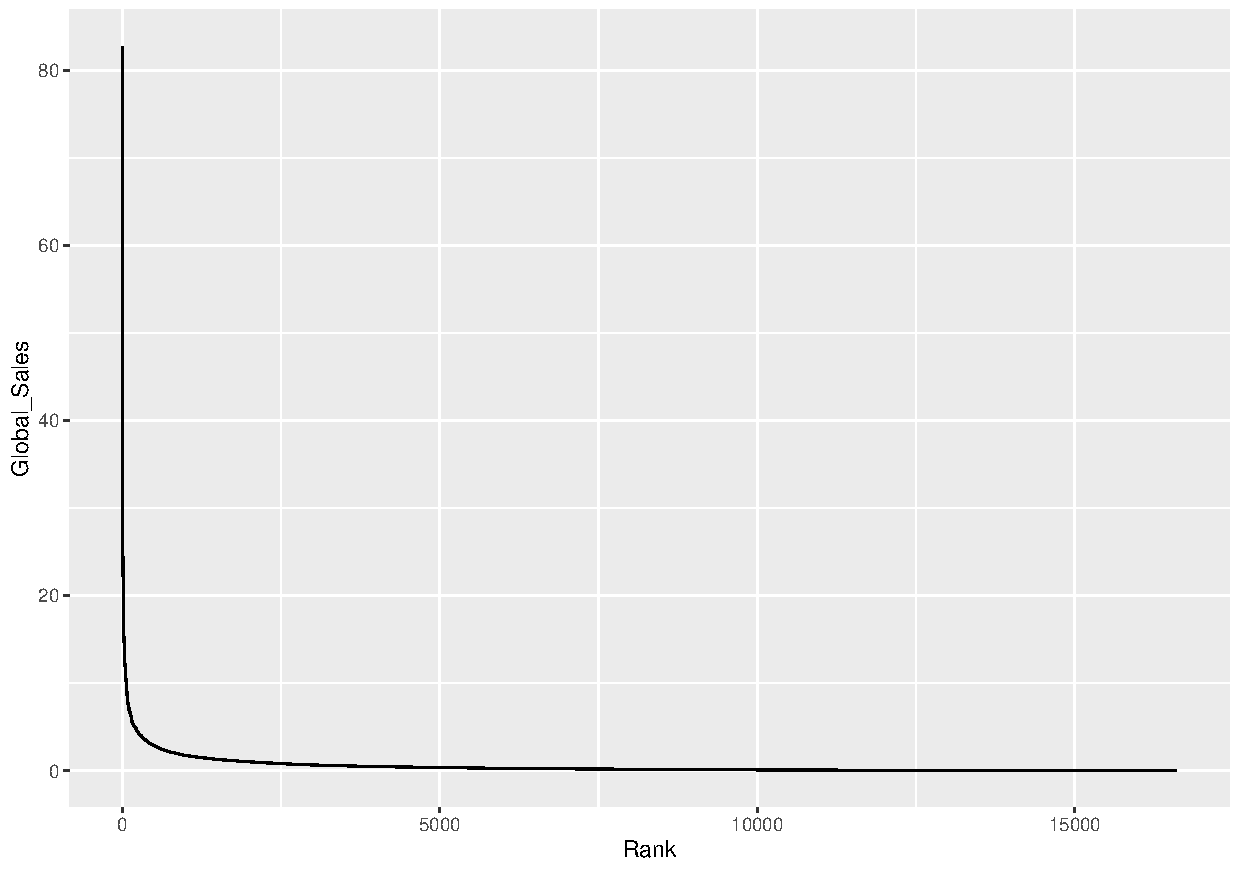
\includegraphics[width=15cm]{\plotsDirectory/1.pdf}
  	\caption{Wykres zależności zmiennej głównej od rangi}
	\end{figure}	
	\end{center}\vspace{1cm}Wykres został wygenerowany za pomocą kodu:
	\begin{lstlisting}[language=R]
ggplot(
  data = data,
  aes(
    y = Global_Sales,
    x = Rank 
  )
)+
  geom_line()
\end{lstlisting}
	\section{Obliczenie podstawowych statystyk opisowych zmiennej głównej}
	
Obliczenia zostały wykonane za pomocą kodu:
	
	\begin{lstlisting}[language=R]
description_statistics = function (data) {
  
  number_of_records = length(data)
  number_of_records_inverted = 1/number_of_records
  
  mean = mean(data)
  
  variance = var(data) * (number_of_records - 1) * number_of_records_inverted
  
  standard_deviation = variance ^ .5
  inside = (data - mean)/standard_deviation
  
  assymetry = sum(inside^3)*number_of_records_inverted
  curtosis  = sum(inside^4)*number_of_records_inverted - 3
  
  c(min, first_quartil, median, third_quartil, max) %<-% fivenum (data)
  
  interquartile_range = third_quartil - first_quartil
  
  quartil_deviation = interquartile_range * .5
  
  mean_quartil = (first_quartil + third_quartil) * .5
  
  quartil_assymetry_coefficient = (mean_quartil - median) / quartil_deviation
  
  quartil_variance_coefficient = quartil_deviation / median * 100
  
  list(
    number_of_records = number_of_records,
    mean = mean,
    standard_deviation = standard_deviation,
    
    assymetry = assymetry,
    curtosis = curtosis,
    
    min = min,
    first_quartil = first_quartil,
    median = median,
    third_quartil = third_quartil,
    max = max,
    
    interquartile_range = interquartile_range,
    quartil_deviation = quartil_deviation,
    mean_quartil = mean_quartil,
    
    quartil_assymetry_coefficient = quartil_assymetry_coefficient,
    quartil_variance_coefficient = quartil_variance_coefficient
  )
}

Global_Sales_stats = description_statistics(Global_Sales)

Global_Sales_stats
\end{lstlisting}
	Uzyskane wyniki\\
	Liczba prób
	$$n(\texttt{Global\_Sales}) = 16598$$
	Średnia
	$$mean(\texttt{Global\_Sales}) = 0.5374407$$
	Odchylenie standardowe
	$$\sigma(\texttt{Global\_Sales}) = 1.554981$$
	Współczynnik asymetrii
	$$A(\texttt{Global\_Sales}) = 17.39907$$
	Kurtoza
	$$K(\texttt{Global\_Sales}) = 603.7501$$
	Wartość minimalna
	$$min(\texttt{Global\_Sales}) = 0.01$$
	Pierwszy kwartyl
	$$Q_1(\texttt{Global\_Sales}) = 0.06$$
	Mediana
	$$M_e(\texttt{Global\_Sales}) = 0.17$$
	Trzeci kwartyl
	$$Q_3(\texttt{Global\_Sales}) = 0.47$$
	Wartość maksymalna
	$$max(\texttt{Global\_Sales}) = 82.74$$
	Rozstęp między kwartylowy
	$$IQR(\texttt{Global\_Sales}) = 0.41$$
	Odchylenie ćwiartkowe
	$$Q(\texttt{Global\_Sales}) = 0.205$$
	Kwartyl średni
	$$\bar{Q}(\texttt{Global\_Sales}) = 0.265$$
	Kwartylny współczynnik asymetrii
	$$A_k(\texttt{Global\_Sales}) = 0.4634146$$
	Kwartylny współczynnik zmienności
	$$V_k(\texttt{Global\_Sales}) = 120.5882$$
	
	\section{Dobór zmiennych (przynajmniej trzech), które mogą mieć wpływ na zmienną główną}
	Do analizy zostały wybrane 3 następujące zmienne.
	\begin{lstlisting}[language=R]
NA_Sales
EU_Sales
JP_Sales
\end{lstlisting}
Te zmienne mogą pozwolić ustalić który region ma najważniejszy wpływ na globalną sprzedaż.
	\section{Graficzna prezentacja wybranych w poprzednim kroku zmiennych}
	Na poniższych wykresach zostały przedstawione zmienne (wybrane w poprzednim punkcie) w zależności od rangi wiodącej.\\
	Wykresy zostały uzyskane za pomocą poniższego kodu:
	\begin{lstlisting}[language=R]
ggplot(
  data = data,
  aes(
    y = NA_Sales,
    x = Rank 
  )
)+
  geom_line()

ggplot(
  data = data,
  aes(
    y = EU_Sales,
    x = Rank 
  )
)+
  geom_line()

ggplot(
  data = data,
  aes(
    y = JP_Sales,
    x = Rank 
  )
)+
  geom_line()
\end{lstlisting}
	\begin{center}
	\begin{figure}[H]
  	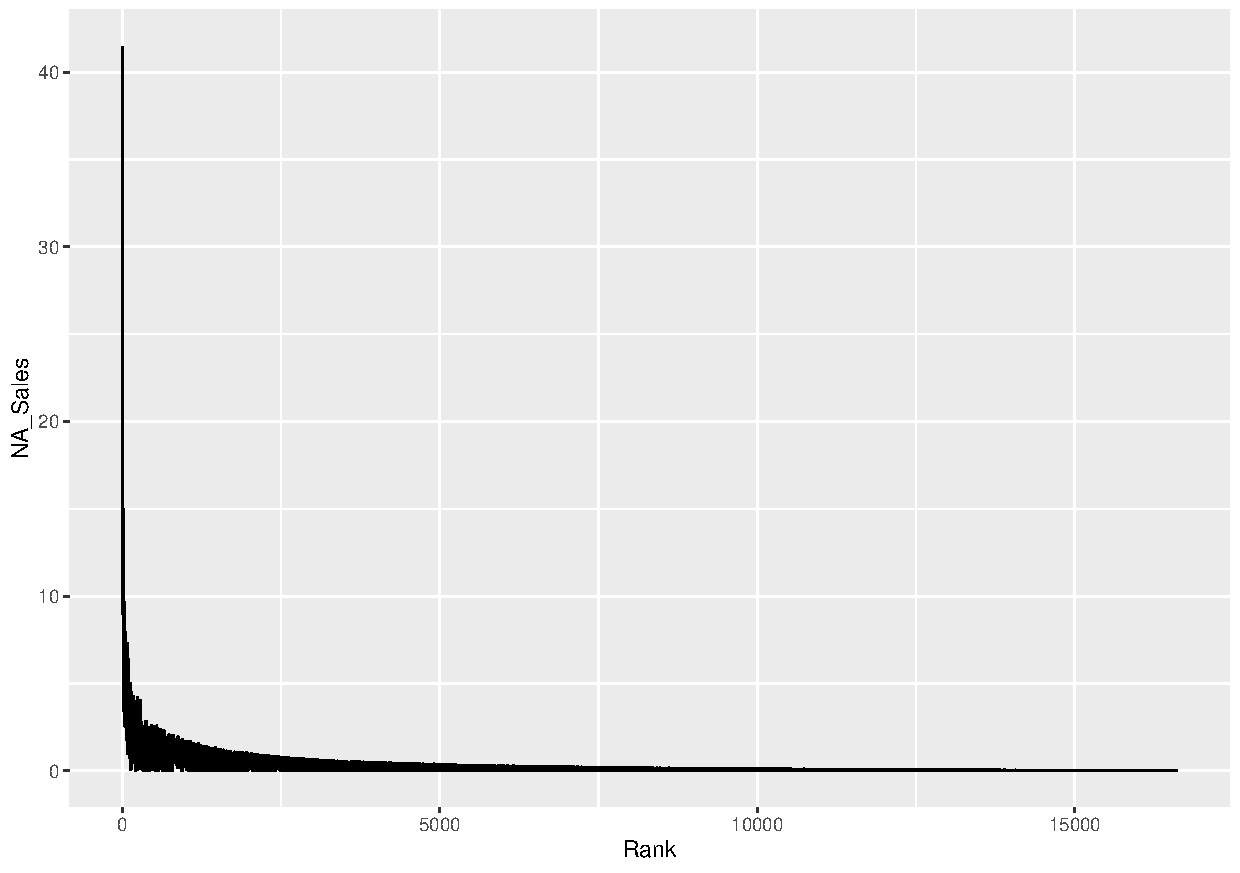
\includegraphics[width=15cm]{\plotsDirectory/2.pdf}
  	\caption{Wykres zależności zmiennej \texttt{NA\_Sales} od rangi}
	\end{figure}	
	\begin{figure}[H]
  	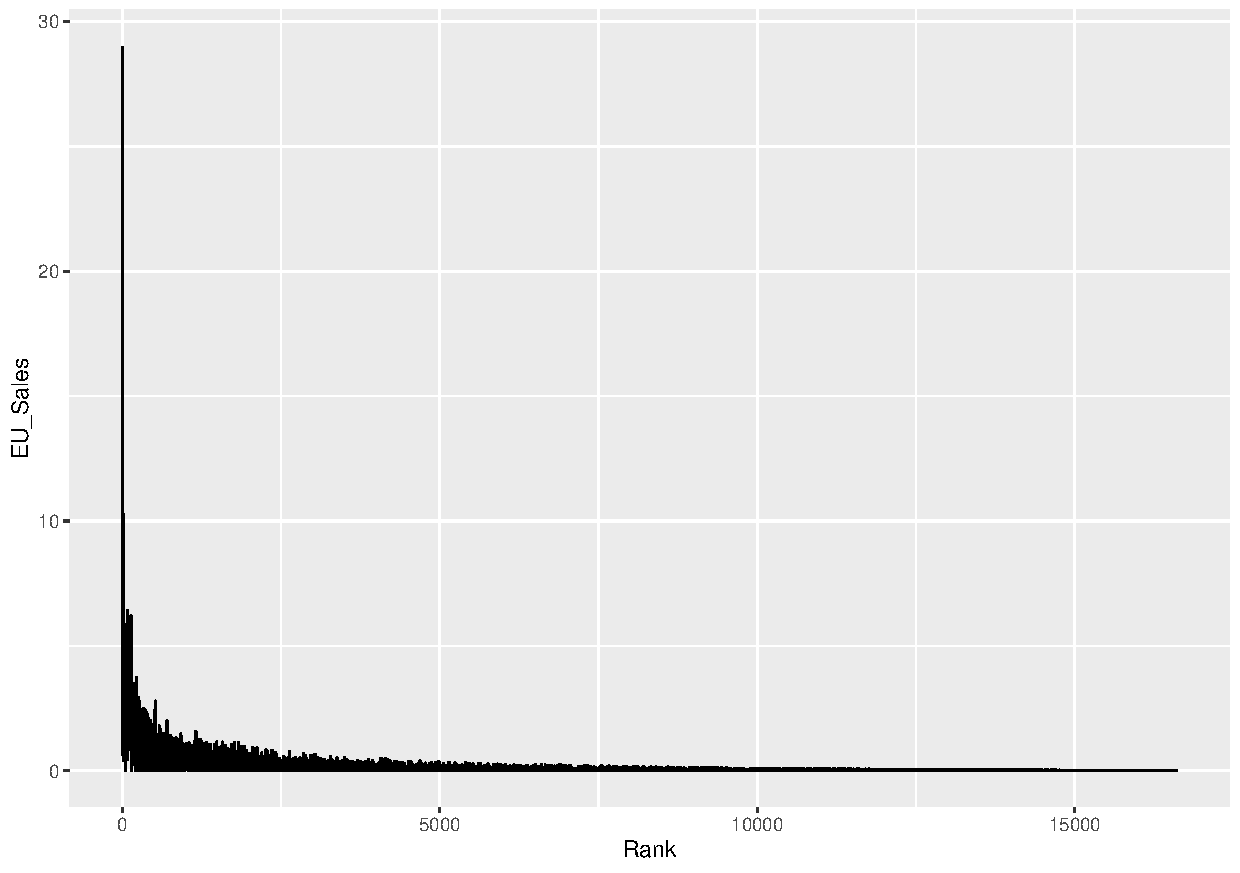
\includegraphics[width=15cm]{\plotsDirectory/3.pdf}
  	\caption{Wykres zależności zmiennej \texttt{EU\_Sales} od rangi}
	\end{figure}	
	\begin{figure}[H]
  	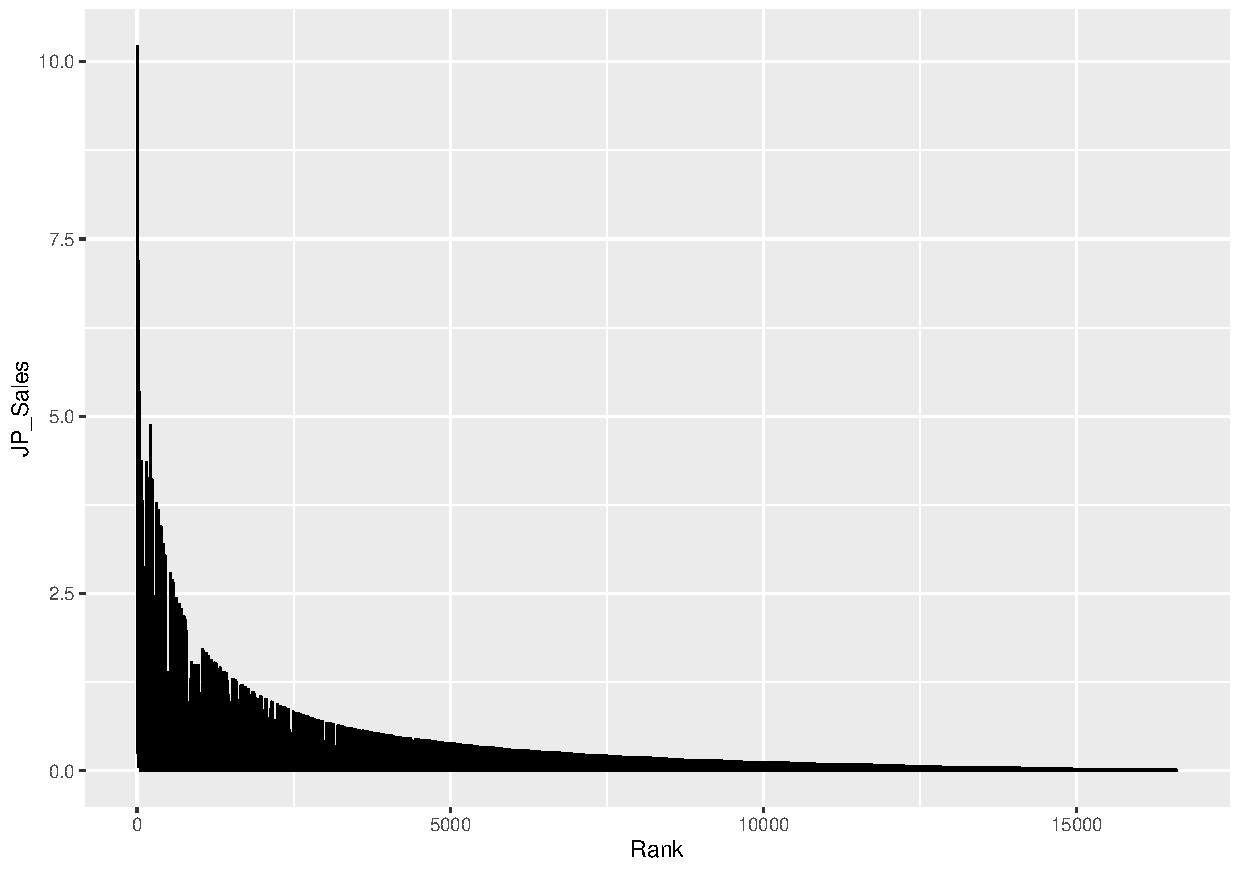
\includegraphics[width=15cm]{\plotsDirectory/4.pdf}
  	\caption{Wykres zależności zmiennej \texttt{JP\_Sales} od rangi}
	\end{figure}	
	\end{center}
	
	\section{Charakterystyka powyższych zmiennych (statystyki opisowe lub rozkłady liczebności, w zależności od klasy zmiennych)}
	Wyniki przedstawione w tabeli zostały uzyskane za pomocą poniższego kodu:
		\begin{lstlisting}[language=R]
NA_Sales_stats = description_statistics(NA_Sales)

EU_Sales_stats = description_statistics(EU_Sales)

JP_Sales_stats = description_statistics(JP_Sales)

NA_Sales_stats

EU_Sales_stats

JP_Sales_stats
\end{lstlisting}
	\begin{center}
	\begin{tabular}{|c|c|c|c|}
	\hline
	\texttt{data} & \texttt{NA\_Sales} &  \texttt{EU\_Sales} &  \texttt{JP\_Sales}\\
	\hline
	$n(\texttt{data})$ & 16598 & 16598 & 16598\\
	\hline
	$mean(\texttt{data})$ & 0.2646674 & 0.146652 & 0.07778166\\
	\hline
	$\sigma(\texttt{data})$ & 0.8166584 & 0.505336 & 0.3092813\\
	\hline
	$A(\texttt{data})$ & 18.79793 & 18.87383 & 11.20545\\
	\hline
	$K(\texttt{data})$ & 648.9344 & 755.7997 & 194.1751\\
	\hline
	$min(\texttt{data})$ & 0 & 0 & 0\\
	\hline
	$Q_1(\texttt{data})$ & 0 & 0 & 0 \\
	\hline
	$M_e(\texttt{dat})$ & 0.08 & 0.02 & 0\\
	\hline
	$Q_3(\texttt{data})$ & 0.24 & 0.11 & 0.04\\
	\hline
	$max(\texttt{data})$ & 41.49 & 29.02 & 10.22\\
	\hline
	$IQR(\texttt{data})$ & 0.24 & 0.11 & 0.04 \\
	\hline
	$Q(\texttt{data})$ & 0.12 & 0.055 & 0.02\\
	\hline
	$\bar{Q}(\texttt{data})$ & 0.12 & 0.055 & 0.02\\
	\hline
	$A_k(\texttt{data})$ & 0.3333333 & 0.6363636 & 1\\
	\hline
	$V_k(\texttt{data})$ & 150 & 275 & Inf\\
	\hline
\end{tabular}	
	\end{center}
	\section{Graficzna prezentacja zależności}
	Wykresy zostały uzyskane za pomocą poniższego kodu:
	\begin{lstlisting}[language=R]
ggplot(
  data = data,
  aes(
    y = NA_Sales,
    x = Global_Sales
  )
)+
  geom_point()

ggplot(
  data = data,
  aes(
    y = EU_Sales,
    x = Global_Sales
  )
)+
  geom_point()

ggplot(
  data = data,
  aes(
    y = JP_Sales,
    x = Global_Sales
  )
)+
  geom_point()
\end{lstlisting}
	\begin{center}
	\begin{figure}[H]
  	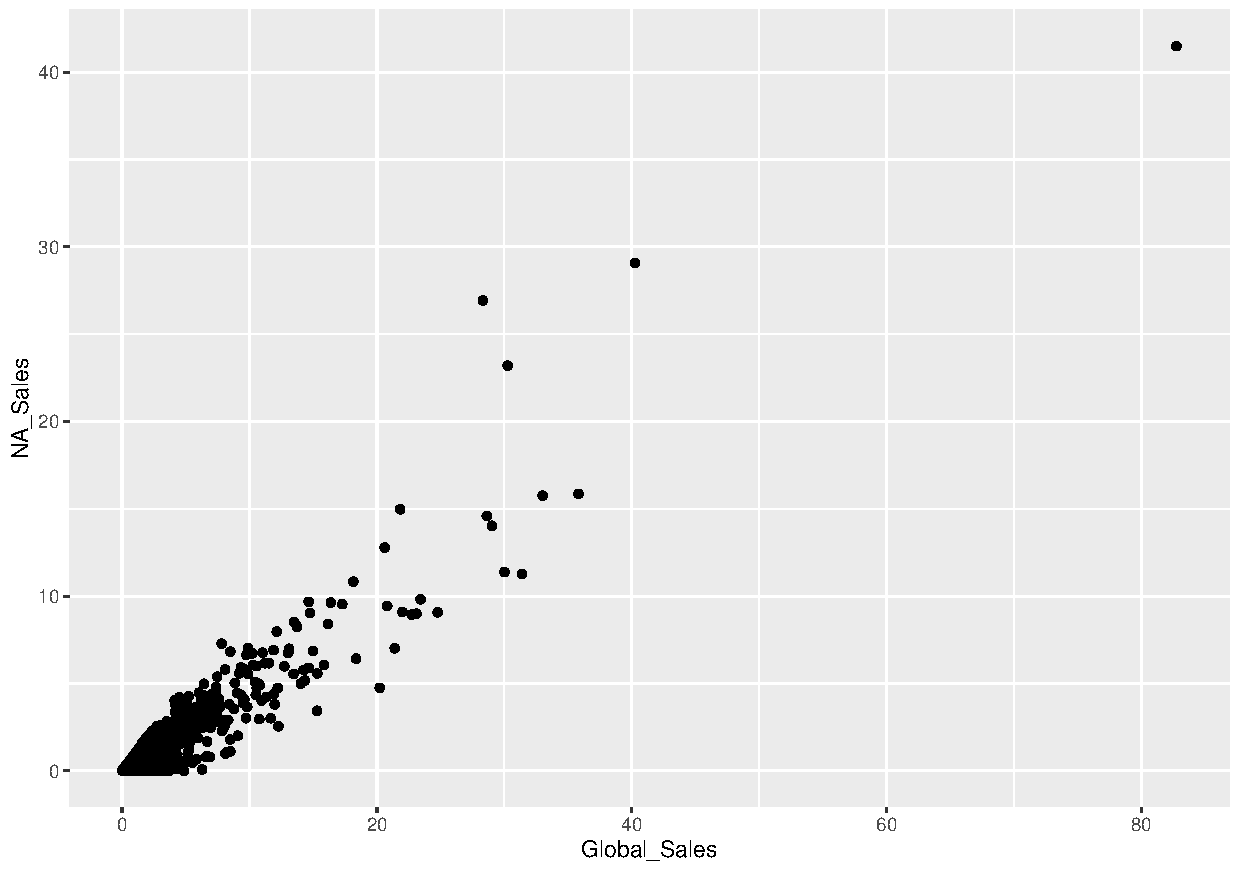
\includegraphics[width=15cm]{\plotsDirectory/5.pdf}
  	\caption{Wykres zależności zmiennej \texttt{NA\_Sales} od \texttt{Global\_Sales}}
	\end{figure}	
	\begin{figure}[H]
  	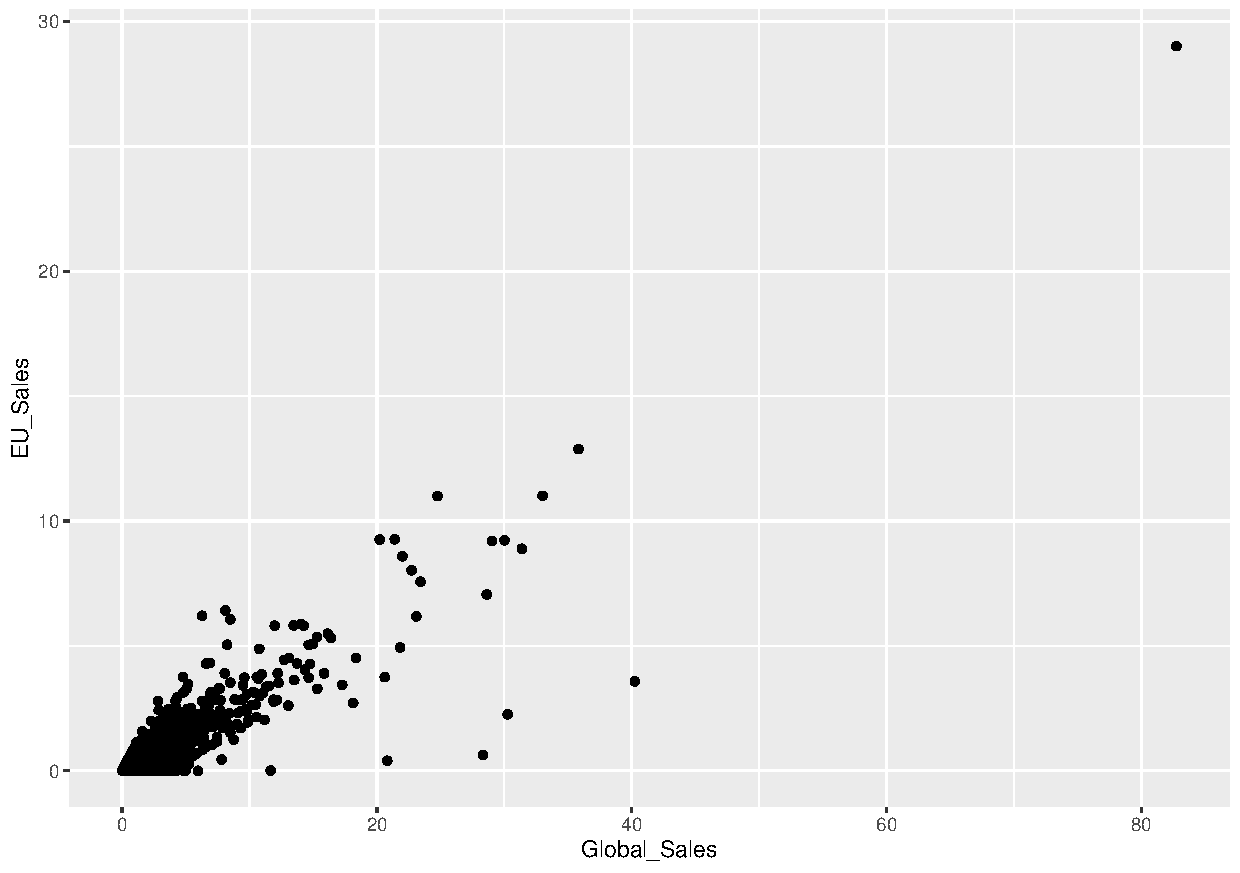
\includegraphics[width=15cm]{\plotsDirectory/6.pdf}
  	\caption{Wykres zależności zmiennej \texttt{EU\_Sales} od \texttt{Global\_Sales}}
	\end{figure}	
	\begin{figure}[H]
  	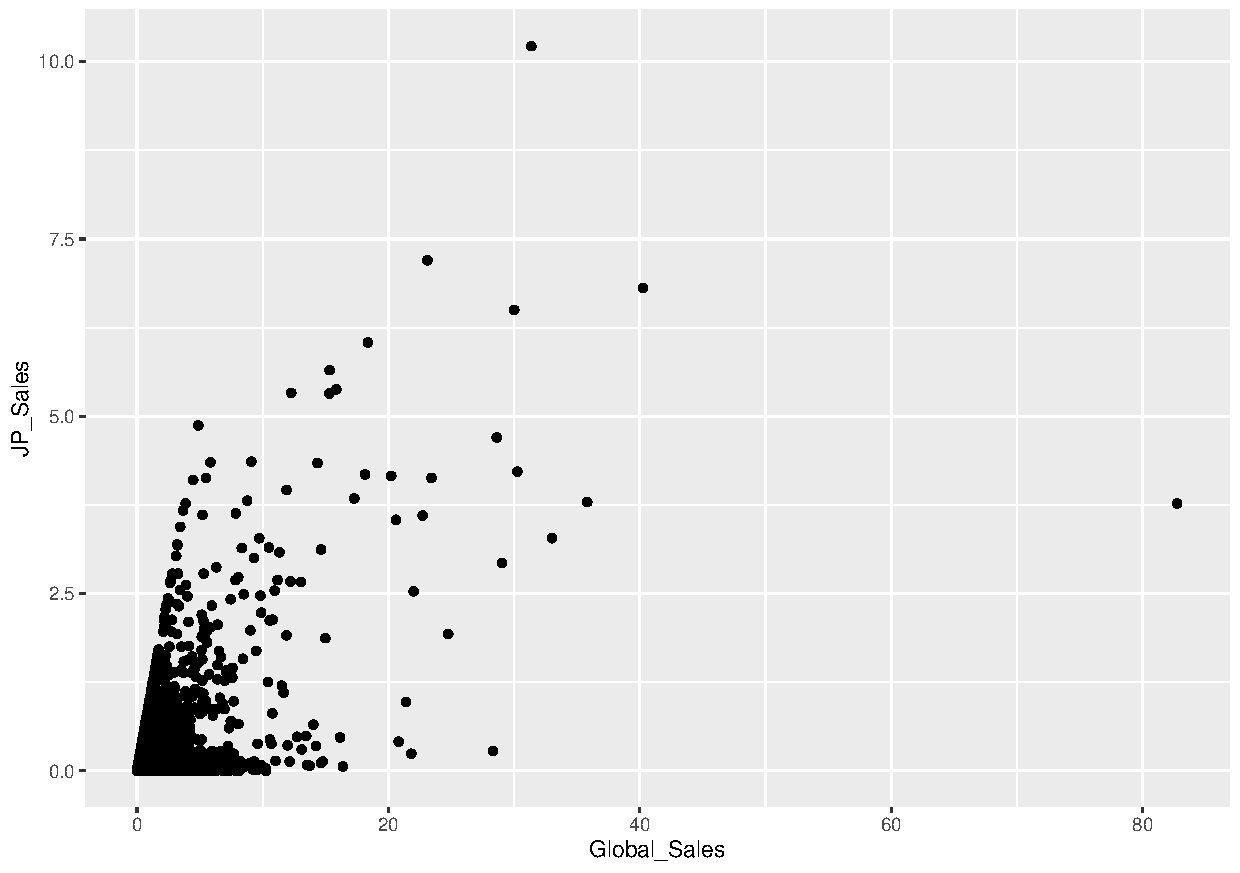
\includegraphics[width=15cm]{\plotsDirectory/7.pdf}
  	\caption{Wykres zależności zmiennej \texttt{JP\_Sales} od \texttt{Global\_Sales}}
	\end{figure}	
	\end{center}	
	
	\section{Wykonanie odpowiedniego testu statystycznego, który potwierdzi lub odrzuci hipotezę o zależności}
	
	W celu sprawdzenia korelacji między wybranymi zmiennymi a zmienną główną przeprowadzony został test Spearmana za pomocą poniższego kodu.
	\begin{lstlisting}[language=R]
spearman_test = function(data) {
  cor.test(Global_Sales, data, method = "spearman", exact = F)
}
spearman_test(NA_Sales)

spearman_test(EU_Sales)

spearman_test(JP_Sales)
\end{lstlisting}
Współczynniki dla poszczególnych przypadków przedstawiają się w następujący sposób:
$$\rho(\texttt{Global\_Sales},\texttt{NA\_Sales}) = 0.7955717$$
$$\rho(\texttt{Global\_Sales},\texttt{EU\_Sales}) = 0.6968457$$
$$\rho(\texttt{Global\_Sales},\texttt{JP\_Sales}) = 0.1519311$$
\section{Wnioski}
	Z wyników testu Spearmana wynika, że najbardziej skorelowaną zmienną ze zmienną główną jest \texttt{NA\_Sales}. Wykres przedstawiony na rysunku 7 również zdaje się potwierdzać tę hipotezę (ze względu na widoczną niemalże liniową zależność). Ze statystyk opisanych w punkcie 6 można wywnioskować, że najmniej ze wszystkich gier w tym zestawieniu sprzedało się na rynku japońskim. Wykres przedstawiony na rysunku 4 przedstawia najbardziej wahające się wartości ze wszystkich wybranych zmiennych. Może być to spowodowane niedostępnością niektórych z gier na rynku japońskim.\\
	Wszystkie z przedstawionych zmiennych zdają się (w uśrednieniu) rosnąć hiperbolicznie względem rangi.
	\begin{thebibliography}{1}
    \addcontentsline{toc}{chapter}{Bibliografia}
    \bibitem{source}
    \url{https://www.kaggle.com/datasets/gregorut/videogamesales}
    
    [dostęp: 13.06.2022 22:37 GMT+2]
\end{thebibliography}
\end{document}